%\documentclass[ignorenonframetext, compress, 9pt, xcolor=svgnames]{beamer} 
\input{../Config_diapos}
\usepackage{color}
\usepackage{tikz}
\usetikzlibrary{shapes.geometric, arrows}
\usepackage{enumerate}   
\usepackage{multirow}
\usepackage{txfonts}
\usepackage{mathrsfs}
\usepackage{appendixnumberbeamer}
%\setbeamersize{text margin left=1.5em,text margin right=1.5em} 
%\setbeamersize{text margin left=1.2cm,text margin right=1.2cm} 
\setbeamersize{text margin left=1.5em,text margin right=1.5em} 
%\usepackage{xr}
%\externaldocument{Econometrie1_UGA_P2e}
  \usepackage{eso-pic}
%\newcommand\AtPagemyUpperLeft[1]{\AtPageLowerLeft{%
%\put(\LenToUnit{0.9\paperwidth},\LenToUnit{0.85\paperheight}){#1}}}
%\AddToShipoutPictureFG{
 % \AtPagemyUpperLeft{{\includegraphics[width=1.1cm,keepaspectratio]{logoUGA2020.pdf}}}
%}%

%\setbeamercolor{title}{fg=black}
%\setbeamercolor{frametitle}{fg=black}
%\setbeamercolor{section in head/foot}{fg=black}
%\setbeamercolor{author in head/foot}{bg=Brown}
%\setbeamercolor{date in head/foot}{fg=Brown}
\setbeamertemplate{section page}
{
    \begin{centering}
    \begin{beamercolorbox}[sep=11pt,center]{part title}
    \usebeamerfont{section title}\thesection.~\insertsection\par
    \end{beamercolorbox}
    \end{centering}
}
%\titlegraphic{\includegraphics[width=1cm]{logoUGA2020.pdf}}
\title[Regression linéaire]{\textbf{ \'ECONOM\'ETRIE \\ (UGA, S2)}}
\subtitle{\textbf{CHAPITRE 3:\\ ENDOGÉNÉITÉ ET VARIABLES INSTRUMENTALES(1)}}
\date{\today}
\author{Michal W. Urdanivia\inst{*}}
\institute{\inst{*}UGA, Facult\'e d'\'Economie, GAEL, \\
e-mail:
 \href{
     mailto:michal.wong-urdanivia@univ-grenoble-alpes.fr}{michal.wong-urdanivia@univ-grenoble-alpes.fr}}

%\titlegraphic{\includegraphics[width=1cm]{logoUGA2020.pdf}
%}

\begin{document}

%%% TIKZ STUFF
\usetikzlibrary{positioning}
\usetikzlibrary{snakes}
\usetikzlibrary{calc}
\usetikzlibrary{arrows}
\usetikzlibrary{decorations.markings}
\usetikzlibrary{shapes.misc}
\usetikzlibrary{matrix,shapes,arrows,fit,tikzmark}
\usetikzlibrary{shapes}
\usetikzlibrary{shapes.geometric, arrows}
\tikzset{   
        every picture/.style={remember picture,baseline},
        every node/.style={anchor=base,align=center,outer sep=1.5pt},
        every path/.style={thick},
        }
\newcommand\marktopleft[1]{
    \tikz[overlay,remember picture] 
        \node (marker-#1-a) at (-.3em,.3em) {};%
}
\newcommand\markbottomright[2]{%
    \tikz[overlay,remember picture] 
        \node (marker-#1-b) at (0em,0em) {};%
}
\tikzstyle{every picture}+=[remember picture] 
\tikzstyle{mybox} =[draw=black, very thick, rectangle, inner sep=10pt, inner ysep=20pt]
\tikzstyle{fancytitle} =[draw=black,fill=red, text=white]
\tikzstyle{observed}=[draw,circle,fill=gray!50]

\begin{frame}
\titlepage
\end{frame}
\begin{frame}
 \tableofcontents
    \end{frame}
%\begin{frame}
%\frametitle{Contenu}
%\tableofcontents[pausesections, pausesubsections]
%\end{frame}

%\section{Qu'est-ce que l’économétrie ? A quoi (à qui) ça sert ?}
%\frame{\sectionpage}
%\begin{frame}
%  \tableofcontents  
%\end{frame}

\section{Variables explicatives endogènes et biais d'endogénéité}
\frame{\sectionpage}

\begin{frame}[allowframebreaks]{Endogénéité}
\begin{itemize}
\item Nous continuons à étudier un modèle linéaire de forme: 
\begin{align*}
    y_i &=\boldx_i^\prime\bolda_0 + u_i, \ \Exp[u_i]\equiv 0.
\end{align*}
où $\dim(\boldx_i) = K$, et on souhaite estimer $\bolda_0$.
\item Dans le chapitre précédent il a été montré qu'une condition essentielle 
pour l'identification  de $\bolda_0$ et son estimation convergente par les MCO est que  $\boldx_i$ 
soit exogène:
\begin{align*}
 \underbrace{\Exp[u_i|\boldx_i] = 0}_{\text{exogénéité forte}} &\Rightarrow
 \underbrace{\Exp[\boldx_iu_i] = \Cov[\boldx_i; u_i] = 0}_{\text{exogénéité faible}}.
\end{align*}
\item Inversement quand $\Exp[\boldx_iu_i] \neq 0$ on parle d'endogénéité des variables explicatives.
\item Il convient néanmoins de noter $\Exp[\boldx_iu_i] \neq 0$ peut être du à seulement 
certains éléments de $\boldx_i$, par exemple:
\begin{enumerate}[$\star$]
\item On peut avoir $M\in\{0, \ldots, K\}$ éléments de $\boldx_i$ tels que $\Exp[x_{k, i}u_i] = 0, \ k = 1, \ldots, M.$, 
et ces variables seront qualifiées d'exogènes.
\item Alors que les $K-M$ autres éléments de $\boldx_i$ sont tels que  $\Exp[x_{k, i}u_i] \neq 0 , \ k = M + 1, \ldots, K$,
et ces variables seront qualifiées d'endogènes.
\end{enumerate}

\end{itemize}
\end{frame}
\begin{frame}[allowframebreaks]{Non convergence de l'estimateur des MC en présence d'endogénéité}
\begin{itemize}
     \item Les résultats du chapitre précédent nous permettent d'écrire que 
     pour l'estimateur des MCO de $\bolda_0$ 
     que:
     \begin{align*}
         \underset{N\to +\infty}{\plim}\hat{\bolda}_N^{MCO} &=    \left\{
            \begin{array}{ll}
         \bolda_0 + \underbrace{\Exp[\boldx_i\boldx_i]^{-1}\Exp[\boldx_iu_i]}_{=0} = \bolda_0
         &\text{quand $\boldx_i$ est exogène},\\
         \bolda_0 + \underbrace{\Exp[\boldx_i\boldx_i]^{-1}\Exp[\boldx_iu_i]}_{\neq 0} \neq \bolda_0
&\text{quand $\boldx_i$ est endogène},
        \end{array}
        \right.
     \end{align*}
où le terme $\Exp[\boldx_i\boldx_i]^{-1}\Exp[\boldx_iu_i]$ est le biais (asymptotique) 
d’endogénéité de l'estimateur des MCO de $\bolda_0$.
      \item Poursuivant ce qui a été remarqué plus haut quant au fait d'avoir $\Exp[\boldx_iu_i]\neq 0$, 
      il est important de remarquer que même si une seule variable explicative est
      endogène, disons le $K$-ième élément de $\boldx_i$, $x_{K, i}$, avec donc:
      \[\Exp[x_{K, i}u_i]\neq 0, \quad \text{et} \quad \Exp[x_{k, i}u_i]\neq 0, \quad
      \text{pour $k = 1, \ldots, K-1$}, \]
      alors:
      \begin{enumerate}[$\star$]
        \item Le coefficient estimé de $x_{K, i}$, $\hat{a}^{MC0}_{K, N}$, n'est 
        pas le seul élément de $\hat{\bolda}_N^{MCO}$ potentiellement biaisé.
        \item En général le problème d’endogénéité de $x_{K,i}$ « contamine » les
        les coefficients estimés des autres éléments de $\boldx_i$, $\hat{a}^{MC0}_{k, N}$ 
        pour $k=1, \ldots, K-1$.
        \item Ceci donne une idée de l'importance d'un problème d'endogénéité posé par une 
        ou plusieurs variables explicatives.
      \end{enumerate}
    \end{itemize}
\framebreak 
\begin{remark_fr}
\begin{enumerate}[$\star$]
\item On peut préciser le dernier point précédent. Pour cela
 réécrivons le modèle linéaire:
\begin{align*}
    y_i &= \boldx_{-K, i}^\prime\bolda_{-K, 0} + a_{K, 0}x_{K, i} + u_i, 
    \quad \text{avec} \quad \Exp[\boldx_{-K, i} u_i] = \Exp[u_i]\equiv 0,
\end{align*}
où $\boldx_{-K, i}$ est le vecteur des $K-1$ variables explicatives autres que $x_{K, i}$, 
et $\bolda_{-K, 0}$ leurs coefficients respectifs.
\item En utilisant le propriétés des projections linéaires(c.f., chapitre 2) 
on obtient l'équation suivante,
 $\hat{\bolda}_{N}^{MCO} \equiv (\hat{\bolda}_{-K, N}^{MCO} , \hat{a}^{MC0}_{K, N})$, de
  $\bolda \equiv (\bolda_{-K, 0} ,a_{K, 0})$ dû 
à l’endogénéité de $x_{K, i}$:
\begin{align*}
\plim \hat{\bolda}_N^{MC0}&=\bolda_0 + \underbrace{\Cov[x_{K, i}; u_i]\times \Vr[e_{K, i}]
\times \begin{bmatrix}
    -\boldgamma_K\\
    1
\end{bmatrix}
}_{\text{Biais as. de $\hat{\bolda}_N^{MC0}$} },
\end{align*}
où $e_{K, i} \equiv x_{K, i}-\EL[x_{K, i}| \boldx_{-K, i}]$ 
est le résidu de la projection linéaire de  $x_{K, i}$ sur $\boldx_{-K, i}$: 
$\boldx_{-K, i}^\prime\boldgamma_K\equiv \EL[x_{K, i}| \boldx_{-K, i}]$.
\item Sont donc biaisés asymptotiquement:  $\hat{a}^{MC0}_{K, N}$, 
les éléments de $\hat{\bolda}_{-K, N}^{MCO}$ correspondant aux éléments de $\boldx_{-K, i}$ 
liés à $x_{K, i}$(au sens où leurs coefficients dans $\boldgamma_K$ sont non nuls),
 et la constante du modèle.
\end{enumerate}

\end{remark_fr}
\end{frame}

\section{Sources de l'endogénéité}
\frame{\sectionpage}

\begin{frame}[allowframebreaks]{Pourquoi peut t-il y avoir un problème d'endogénéité?}
\begin{itemize}
    \item On présente par des exemples, les cas dans lesquels on peut avoir $\Exp[\boldx_iu_i] = 0$.
    \item On parle ici de trois formes/sources d'endogénéité:
    \begin{enumerate}
        \item Variables explicatives pertinentes omises. 
        \item Simultanéité. 
        \item Erreurs de mesure sur les variables explicatives.
    \end{enumerate}
    \item Dans tous ces cas, qui ne sont pas exclusifs les uns par rapport aux autres, 
    les MCO ne sont pas convergents.
\end{itemize}
\end{frame}

\begin{frame}[allowframebreaks]{Variables explicatives pertinentes omises}
\begin{itemize}
\item On s'appuie ici sur les travaux de \cite{angrist1991}, et \cite{card1993} 
qui s'intéressent à la mesure de l'effet causal du niveau d'études sur le salaire. 
\item Pour cela ils considèrent une équation linéaire du type: 
\begin{align}
    lwage_i&= \alpha_0 + b_{1, 0}educ_i + \boldc_i^\prime\boldb_{-1, 0} + u_i, \quad 
    \text{avec} \quad \Exp[\boldc_iu_i] = \Exp[u_i]\equiv 0,
    \label{eq11}
\end{align}
où pour un individu $i$ dans la population de référence:
\begin{enumerate}[$\star$]
\item $lwage_i$ est son salaire annuel en logarithme.
\item $educ_i$ le nombre d'années études réalisés.
depuis l'entrée dans le primaire.
\item $\boldc_i$ est un vecteur 
d'autres caractéristiques observées de l'individu et corrélées avec son salaire. 
Par exemple son lieu de résidence, 
son expérience professionnelle en nombre d'années, son origine ethnique, etc. 
Ces caractéristiques sont supposées exogènes.
\end{enumerate}
\item Un problème courant dans cette littérature concerne l'\emph{ability bias}. 
\end{itemize}
\framebreak

\begin{itemize}
    \item Citons \cite{card1993}:
%\begin{columns}[T] % align columns
%\hfill%
%\begin{column}{.6\textwidth}
\begin{mdframed}

    \begin{center}
  \includegraphics[width=.6\textwidth]{cardNBER19931.png}
    \end{center}
    
\end{mdframed}
%\end{column}%
%\hfill%
%\end{columns}
            \item Où le terme $\beta$ correspond au coefficient de $educ_i$ que nous avons noté $\boldb_{1, 0}$ dans 
            \eqref{eq11}.
            \item Notons la caractéristique inobservée que l'auteur appelle \emph{ability}(que l'on peut essayer de
             traduire par capacité ou compétence) $abil_i$.
            \item Suivant l'auteur on s'attend à ce que $abil_i$:
            \begin{enumerate}[$\star$]
            \item ait un effet positif sur $lwage_i$, 
            \item soit corrélée positivement avec $educ_i$. 
            \end{enumerate}
            \item On peut résumer cela par deux équations.
            \begin{enumerate}[$\star$]
            \item La première inclut l'effet de la caractéristique inobservé $abil_i$ dans l'erreur 
            du modèle \eqref{eq11}:
            \begin{align}
                lwage_i&= \alpha_0 + b_{1, 0}educ_i + \boldc_i^\prime\boldb_{-1, 0} 
                + \underbrace{\delta_0 abil_i + v_i}_{u_i}, 
                \quad \text{avec} \quad \Exp[v_i | educ_i, \boldc_i, abil_i] = \Exp[v_i]\equiv 0,
                \label{eq12}
            \end{align}
            \item La seconde prend en compte la corrélation entre $abil_i$ et $educ_i$ en considérant 
            l'équation de la projection linéaire de $educ_i$ sur $abil_i$ et une constante.
            \begin{align}
                educ_i &= \gamma_0 + \gamma_1abil_i + r_i, \quad \text{avec} \quad 
                \Exp[r_i abil_i] = 0.
                \label{eq13}
            \end{align}
            où $r_i$ est le résidu de cette projection, et on sait que $\gamma_1 = 
            \frac{\Cov[educ_i; abil_i]}{\Vr[abil_i]}$.
        \end{enumerate}
        \item En résumé, si on observait $abil_i$ un estimateur convergent de $b_{1, 0}$ 
        serait l'estimateur des MCO de l'équation dans \eqref{eq12}, mais comme $abil_i$ 
        est inobservée on estime l'équation dans \eqref{eq11} dont l'erreur inclut $abil_i$. 
        \item Mais dans ce cas nous avons, 
        \begin{align*}
            \Cov[educ_i; u_i] &= \Cov[\gamma_0 + \gamma_1abil_i + r_i; \delta_0 abil_i + v_i]\\
            &= \gamma_1\delta_0 \Vr[abil_i].
        \end{align*}
        \item Par conséquent, $educ_i$ est endogène dans le modèle \eqref{eq11} sauf si: 
        \begin{enumerate}[$\star$]
            \item $\gamma_1 = 0$ auquel cas $abil_i$ et $educ_i$ ne sont pas corrélés,
            \item ou $\delta_0 = 0$ auquel cas $abil_i$ n'est pas pertinente comme explicative de $lwage_i$.
        \end{enumerate}
    \end{itemize}

\end{frame}

\begin{frame}[allowframebreaks]{Simultanéité}
\begin{itemize}
    \item On considère comme exemple le travail de \cite{angrist1998} sur l’effet de la maternité(nombre d'enfants) 
    sur l'offre de travail(nombre d'heures travaillées).
    \item Il est vraisemblable que les choix de maternité et les choix professionnels soient décidés conjointement, 
    et que par conséquent les deux propositions suivantes soient « vraies » :
    \begin{enumerate}[$\star$]
    \item Le salaire est un déterminant du nombre d'enfants selon un double effet « ressources » et
    « temps disponible » pour les enfants.
    \item Le nombre d'enfants est un déterminant du salaire selon double effet « ressources » et
    « temps disponible » pour la carrière professionnelle.
    \end{enumerate}
    \item Cette simultanéité peut être analysée dans le 
    cadre du système d'équations linéaire suivant:
    \begin{align*}
        \left\{
        \begin{array}{ll}
    heures_i &= a_{1, 0}enfants_i + \boldx_{-1, i}^\prime\bolda_{-1, 0} + u_i,\\
    enfants_i &= \alpha_{1, 0} heures_i + \boldz_{-1, i}^\prime\boldalpha_{-1, 0} + v_i,
        \end{array}
        \right.
    \end{align*}
    où $heures_i$ est le nombre d'heures travaillées par semaine, $enfants_i$ est le 
    nombre d'enfants dans une famille, 
    $\boldx_{-1, i}$ et  $\boldz_{-1, i}$  sont des 
    vecteur de variables explicatives exogènes(incluant chacun un régresseur 
    constant) pour respectivement le nombre d'heures travaillées par semaine, 
    et le nombre d'enfants.
    
    \item En substituant l'expression pour les heures dans
     l'équation pour le nombre d'enfants, nous obtenons(en supposant 
     que $1- a_{1, 0}\alpha_{1, 0}\neq 0$),
    \begin{align*}
    enfants_i  = \boldx_{-1, i}^\prime\left(\frac{\bolda_{-1, 0}
    \alpha_{1, 0}}{1-a_{1, 0}\alpha_{1, 0}}\right) + \boldz_{-1, i}^\prime
     \left(\frac{\boldalpha_{-1, 0}}{1-a_{1, 0}\alpha_{1, 0}}\right) + 
     \left(\frac{\alpha_{1, 0}}{1-a_{1, 0}\alpha_{1, 0}}\right)u_i + 
     \left(\frac{1}{1-a_{1, 0}\alpha_{1, 0}}\right)v_i
    \end{align*}
    En supposant que $\boldx_{-1, i}$, $\boldz_{-1, i}$, $v_i$ ne sont pas 
    corrélés avec $u_i$, nous obtenons,
    \begin{align*}
    \Exp(u_ienfants_i) &= \left(\frac{\alpha_{1, 0}}{1-a_{1, 0}\alpha_{1, 0}}\right)\Exp(u_i^2)\neq 0
    \end{align*}

\end{itemize}
\end{frame}

\begin{frame}[allowframebreaks]{Erreurs de mesure sur les variables explicatives}
\begin{itemize}
\item Pour simplifier la présentation on considère le modèle simple suivant:
\begin{align*}
    y_i &= \alpha_0 + b_0\tilde{x}_i +u_i, 
    \quad \text{avec} \quad \Exp[u_i|\tilde{x}_i]= \Exp[u_i]\equiv 0.
\end{align*}
\item Le problème est qu'à la place de $\tilde{x}_i$ on observe une mesure imparfaite 
de cette variable $\tilde{x}_i^e$. 
\item En effet $\tilde{x}_i^e$  est affectée d'erreurs de mesure:
\begin{align*}
    \tilde{x}_i^e &= \tilde{x}_i + \underbrace{e_i}_{\substack{\text{erreur de}\\ 
    \text{mesure}\\\text{sur $\tilde{x}_i$}}} , \quad \text{avec} \quad \Exp[e_i|\tilde{x}_i]= \Exp[u_i|e_i]
    = \Exp[e_i] = 0.
\end{align*}
\item L’erreur de mesure est donc a priori tout-à-fait anodine: elle est sans biais
et n'est liée ni à $\tilde{x}$,ni à $u_i$.
\item Par la suite on utilisera le fait que: 
\begin{align}
    \Vr[\tilde{x}_i^e]&= \Vr[\tilde{x}_i] + \Vr[ e_i ] .
    \label{eq14}
\end{align}
\item Par substitution de $\tilde{x}_i$ par $\tilde{x}_i^e -e_i$ dans 
le modèle d’intérêt on obtient le « modèle observable » :
\begin{align*}
    y_i &= \alpha_0 + b_0\tilde{x}_i^e + \underbrace{v_i}_{u_i-b_0e_i}, 
    \quad \text{avec} \quad \Exp[ v_i ] =0.
\end{align*}
\item La corrélation entre la variable explicative observée $\tilde{x}_i^e$, et l'erreur $v_i$ est:
\begin{align*}
    \Cov[\tilde{x}_i^e;v_i]&=\Cov[\tilde{x}_i +e_i;u_i -b_0e_i]=-b_0\Vr[e_i] \neq 0,
\end{align*}
et ainsi la variable explicative mesurée avec erreur 
est endogène dans le modèle observable, par « construction ».

\item En outre pour l'estimateur des MCO dans le modèle observable nous avons:
\begin{align}
\underset{N\to +\infty}{\plim} \hat{b}_N^{MCO} &= \frac{\Cov[\tilde{x}_i^e; y_i]}{\Vr[\tilde{x}_i^e]},
\label{eq15}
\end{align}
et comme,
\begin{align}
    \Cov[\tilde{x}_i^e; y_i]&=\Cov[\tilde{x}_i^e;b_0\tilde{x}_i^e + v_i]=
    b_0\Vr[\tilde{x}_i^e]+\Cov[\tilde{x}_i^e; v_i],
    \label{eq16}
\end{align}
on obtient en utilisant \eqref{eq14}-\eqref{eq16}:
\begin{align}
    \underset{N\to +\infty}{\plim} \hat{b}_N^{MCO} = b_0\times\frac{\Vr[\tilde{x}_i]}{\Vr[\tilde{x}_i + \Vr[e_i]]}
    &\Rightarrow \abs{ \underset{N\to +\infty}{\plim} \hat{b}_N^{MCO}} < \abs{b_0}.
    \label{eq17}
\end{align}
\item Le résultat \eqref{eq17} est un exemple de biais d’atténuation, à savoir que l'estimateur 
des MCO de $b_0$ dans le modèle observable sous-estime systématiquement $b_0$ en valeur absolue.
\item Ce type de biais ne concerne pas seulement l'endogénéité en raison d'erreurs de mesure
 pouvant aussi concerner les autres cas d'endogénéité.
\end{itemize}
\end{frame}
\section{Introduction à la notion de variable instrumentale}
\frame{\sectionpage}
\begin{frame}[allowframebreaks]{Endogénéité et (non-)identification dans un modèle linéaire simple}
\begin{itemize}
\item On considère ici le modèle linéaire le plus simple :
\begin{align}
    y_i &=\alpha_0 +b_0x_i + u_i \  \text{avec} \ \Exp[u_i]\equiv 0,
    \label{eq1}
\end{align}
mais on considère que l’analyse du PGD indique que $x_i$ est endogène dans ce 
modèle, i.e. que :
\begin{align*}
\Exp[u_i| x_i]\neq 0 &\Rightarrow \Cov[x_i; u_i]\neq 0.
\end{align*}
\item Rappelons que lorsque $x_i$ est exogène et que $\Var[x_i] \neq 0$, on a par l'exogénéité de 
$x_i$:
\begin{align*}
    \Cov[x_i; u_i] = 0 &\Leftrightarrow \Cov[x_i; y_i - \alpha_0 -b_0x_i] =0
     \Rightarrow b_0 = \frac{\Cov[x_i; y_i]}{\Var[x_i]}.
\end{align*}
\item Autrement dit l'exogénéité de $x_i$ permet d'identifier $b_0$(et aussi de $\alpha_0$)
comme une fonction de la distribution des variables observées $y_i$ et $x_i$.
\item Inversement dans la situation que nous considérons dans ce chapitre  $\Cov[x_i; u_i]\neq 0$, 
rend impossible l'identification $b_0$(et aussi celle de $\alpha_0$), et 
la construction d'un estimateur convergent.

\framebreak

\item On peut représenter ce problème en utilisant un
\href{https://en.wikipedia.org/wiki/Causal\_graph}{\textbf{graphe causal}}: 

\begin{figure}[hbt!]
    \centering
    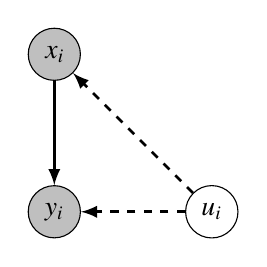
\begin{tikzpicture}
           \node[draw,circle, fill=gray!50](xtilde)  at (0,0) {$x_i$};
          \node[draw,circle,fill=gray!50](y)  at (0,-2) {$y_i$};
      \node[draw,circle](u)  at (2, -2) {$u_i$};
      \draw[->,>=latex, line width= 1] (xtilde) -- (y);
       \draw[->,>=latex, dashed, line width= 1] (u) -- (y);
        \draw[->,>=latex ,dashed,  line width= 1] (u) -- (xtilde);
          \end{tikzpicture}
          \caption{Graphe causal du modèle: $y_i = \alpha_0 + b_0x_i + u_i$, 
          avec $\Cov(x_i ; u_i)\neq 0$. Les variables
          $(x_i, y_i, u_i)$ sont les nœuds du graph et les 
           nœuds foncés correspondent aux variables observées.
          Les arêtes représentent les relations entre les variables. 
          Les relations observées sont en trait plein.}
    \label{fig1}
          \end{figure}
        \end{itemize}
\end{frame}

\begin{frame}[allowframebreaks]{Identification avec une variable instrumentale}
    \begin{itemize}
\item L'intuition sous-jacente à la méthode des VIs consiste à répondre à la question 
de savoir si avec une variable, que nous notons $z_i$, il est possible d'obtenir 
une mesure de la relation causale entre $x_i$ et $y_i$ qui ne dépende pas de $u_i$.
\item Autrement dit, $z_i$ doit être exogène par rapport à $u_i$:
\begin{align}
\Exp[u_i| z_i] = 0 &\Rightarrow \Cov[z_i; u_i]= 0,
    \label{eq2}
\end{align}
ce qui nous permets d'écrire:
\begin{align*}
    \Cov[z_i; u_i]= 0 &\Leftrightarrow 
    \Cov[z_i; y_i - \alpha_0 -b_0x_i] = 0\\
    &\Leftrightarrow \Cov[z_i; y_i - \alpha_0 +b_0\Cov[z_i;x_i] = 0
\end{align*}
\item Ceci indique que pour identifier $b_0$  on doit aussi supposer aussi que,
\begin{align}
\Cov[z_i;x_i]  &\neq 0,
\label{eq3}
\end{align}
et $b_0$ est identifié par:
\begin{align}
b_0 &= \frac{\Cov[z_i; y_i]}{\Cov[z_i;x_i]},
    \label{eq4}
\end{align}
\framebreak

\item On peut résumer les conditions \eqref{eq2}-\eqref{eq3} ainsi: 

\begin{definition_fr}[Conditions de validité de VIs dans un modèle simple]
    Dans le modèle $y_i = \alpha + b_0x_i + u_i$ avec $\Exp[u_i] \equiv 0$ , une variable $z_i$ 
    est un instrument(de $x_i$) ssi:
    \begin{enumerate}[(i)]
\item $\Cov[z_i ;u_i ]= 0$, i.e. $z_i$ est exogène par rapport à $u_i$ et:
\item $\Cov[z_i;x_i]\neq 0 $, i.e. $z_i$ et $x_i$ sont liées.
\end{enumerate}
\end{definition_fr}

\item Dans la représentation en termes de graphe causal cela donne:

\begin{figure}[hbt!]
    \centering
    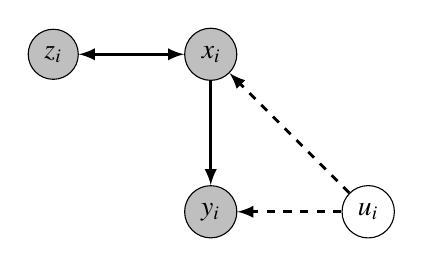
\begin{tikzpicture}
           \node[draw,circle, fill=gray!50](xtilde)  at (0,0) {$x_i$};
           \node[draw,circle,fill=gray!50](ztilde)  at (-2, 0) {$z_i$};
          \node[draw,circle,fill=gray!50](y)  at (0,-2) {$y_i$};
      \node[draw,circle](u)  at (2, -2) {$u_i$};
      \draw[->,>=latex, line width= 1] (xtilde) -- (y);
      \draw[<->,>=latex, line width= 1] (ztilde) -- (xtilde);
       \draw[->,>=latex, dashed, line width= 1] (u) -- (y);
        \draw[->,>=latex ,dashed,  line width= 1] (u) -- (xtilde);
          \end{tikzpicture}
          \caption{Graphe causal du modèle: $y_i = \alpha_0 + b_0x_i + u_i$, 
          avec $\Cov(x_i ; u_i)\neq 0$, $\Cov(z_i ; u_i) = 0$. Les variables
          $(z_i, x_i, y_i, u_i)$ sont les nœuds du graph et les 
           nœuds foncés correspondent aux variables observées.
          Les arêtes représentent les relations entre les variables. 
          Les relations observées sont en trait plein.}
    \label{fig2}
          \end{figure}

\end{itemize}
\end{frame}
\begin{frame}[allowframebreaks]{Estimateur des VIs dans le modèle simple}
    \begin{itemize}
        \item L'identification de $b_0$ par \eqref{eq4} suggère l'estimateur:
        \begin{align}
            \hat{b}_N^{VI} &= \frac{N^{-1}\sumiN(z_i - \bar{z}_N)(y_i - \bar{y}_N)}{
                N^{-1}\sumiN(z_i - \bar{z}_N)(x_i - \bar{x}_N)} = 
                \frac{N^{-1}\sumiN (z_-\bar{z}_N)y_i}
                {N^{-1}\sumiN (z_-\bar{z}_N)x_i},
                \label{eq5}
        \end{align}
        où $\bar{z}_N$, $\bar{x}_N$, et  $\bar{y}_N$ sont le moyennes empiriques respectives de 
        $z_i$, $x_i$, et $y_i$. 
        \item De plus, $\hat{b}_N^{VI}$ est convergent. Nous avons en effet:
        \begin{align*}
            \underset{N\to + \infty}{\plim} N^{-1}\sumiN (z_-\bar{z}_N)y_i &\rightarrow 
            \Cov[z_i; y_i],\\
            \underset{N\to + \infty}{\plim} N^{-1}\sumiN (z_-\bar{z}_N)x_i &\rightarrow 
            \Cov[z_i; x_i],
        \end{align*}
        d'où:
        \begin{align*}
            \hat{b}_N^{VI} \underset{N\to + \infty}{\limp} 
            \frac{\Cov[z_i; y_i]}{\Cov[z_i;x_i]} &= \frac{\Cov[z_i; \alpha_0 + b_0x_i + u_i]}{\Cov[z_i;x_i]},\\
            &= b_0 + \frac{\Cov[z_i;u_i]}{\Cov[z_i;x_i]},\\
            &=b_0.
        \end{align*}
    \end{itemize}
    \framebreak
    \begin{remark_fr}
        \begin{enumerate}[$\star$]
            \item On dit des variations de $z_i$ qu’elles sont des variations exogènes: 
            elles ne sont pas liées à $u_i$ puisque $\Cov[z_i;u_i]=0$.
            \item Ce sont les effets de ces variations exogènes sur $x_i$ qui sont exploitées pour 
            l’identification de $b_0$ grâce à $\Cov[z_i;x_i]\neq 0$.
            \item Noter qu’il n’est aucunement nécessaire que l’effet de $z_i$ sur $x_i$ soit causal. 
            \item L’effet de $z_i$ sur $y_i$ ne « transite » que via $x_i$. 
            La variable instrumentale $z_i$ n’est pas une variable explicative 
            dans le modèle de $y_i$. 
            On parle alors de relation d’exclusion (de la VI $z_i$ vis-à-vis du modèle de $y_i$). 
            \item L'estimateur des VIs est parfois appelé estimateur des moindres carrés indirects. 
            Cela provient de ce que $b_0$ dans $\eqref{eq4}$ peut s'écrire: 
            \begin{align*}
                b_0 &= \frac{\Cov[z_i; y_i] / \Var[z_i]}{\Cov[z_i;x_i] / \Var[z_i]},
                \end{align*}
            qui est le rapport entre le coefficient de $z_i$ dans la projection de $y_i$ sur $z_i$, 
            et le coefficient de $z_i$ dans la projection de $x_i$ sur $z_i$.
        \end{enumerate}
    \end{remark_fr}
    \end{frame}   
\section{L'estimateur de VIs}
\frame{\sectionpage}
\begin{frame}[allowframebreaks]{Variables endogènes, exogènes, instruments}
\begin{itemize}
    \item L’objectif est maintenant de généraliser l’approche présentée dans
     le cas simple précédent au  modèle linéaire général:
    \begin{align}
        y_i&=\boldx_i^\prime\bolda_0 + u_i, \ \text{avec} \ \Exp[u_i] \equiv 0.
        \label{eq6}
    \end{align}
    \item Plusieurs éléments du vecteur $\boldx_i$ 
    peuvent être endogènes de sorte que dans l'estimateur des MCO de $\bolda_0$ plusieurs
    éléments sont potentiellement biaisés(c.f. cours précédent sur les VIs). 
    \item Notons:

    \[\boldx_i = 
    \begin{bmatrix}
        \begin{bmatrix}
        1\\
        \tilde{\boldx}_i^x
        \end{bmatrix}\\
        \tilde{\boldx}_i^e
    \end{bmatrix} 
    =
    \begin{bmatrix}
        \boldx_i^x\\
        \tilde{\boldx}_i^e
    \end{bmatrix}
    \begin{array}{ll}
        \left\{ \text{variables explicatives exogènes}\right. &: \Exp[u_i|x_{k, i}^x] = 0 (k=1,\ldots,M)\\
        \left\{ \text{variables explicatives endogènes}\right.&: \Exp[u_i|x_{k, i}^x] \neq 0(k=M +1,\ldots,K)
    \end{array}
    \]
    \begin{remark_fr}
    \begin{enumerate}[$\star$]
        \item Il est clair que la variable constante $1$ est "exogène" : $\Exp[u_i|1] 
        =\Exp[u_i] =\Exp[1\times ui] =0$.
        \item Comme pour l'estimateur des MCO nous utiliserons la Méthode des Moments 
        pour construire un estimateur convergent de $\bolda_0$ , l’estimateur des VI 
        du modèle \eqref{eq6}.
        \item On considère ici que chaque élément de $\boldx_i^e$ a une variable instrumentale.
    \end{enumerate}
    \end{remark_fr}

    \framebreak
    \begin{definition_fr}[Variable instrumentale]
        $z_{k ,i}$  est une variable instrumentale de $x_{k, i}$ dans le modèle linéaire
         \eqref{eq6} si: 
         \begin{enumerate}[(i)]
            \item $\Cov[z_{k, i}; u_i] = 0$ i.e., $z_{k, i}$ est exogènes par rapport à $u_i$,
            \label{vi1}
            \item $z_{k ,i}$ "suffisamment" liée à $x_{k ,i}$.
            \label{vi2}
         \end{enumerate}
    \end{definition_fr}
    \begin{remark_fr}
        \begin{enumerate}[$\star$]
        \item On verra dans la suite (analyse des conditions de rang) que la condition 
        \eqref{vi2} doit en fait être définie comme:
        \begin{align*}
            \Cov[z_{k, i} ; e_{k, i} ]&\neq 0 \  \text{pour} \ k > 1,
        \end{align*}
        où $e_{k, i}$ est la partie spécifique de $x_{k ,i}$ dans $x_i$ , i.e. 
        le résidu de la projection linéaire de $x_{k ,i}$ sur les autres explicatives $\boldx_{-k, i}$.
        \begin{align*}
            e_{k, i} &= x_{k, i}- \EL[x_{k, i}| \boldx_{-k, i}].
      \end{align*}
      \item Dans la définition d'un VI précédente, on voit que lorsqu'une variable explicative $x_{k, i}$
      est exogène alors c'est aussi une variable instrumentale d'elle même. En ce sens 
      que non seulement elle vérifie \eqref{vi1} mais elle vérifie forcément \eqref{vi2} 
      (car ayant une corrélation de 1 avec elle même)
    \end{enumerate}
    \end{remark_fr}

    \framebreak

    \item On construit le vecteur des variables instrumentales $\boldz_i$ avec:
    
    \[
       \tilde{\boldz}_i^e = 
       \begin{bmatrix} 
        \tilde{z}_{M+1, i}\\
        \tilde{z}_{M+2, i}\\
        \vdots\\
        \tilde{z}_{K, i}
       \end{bmatrix}
       \ \text{et} \
       \boldz_i = 
       \begin{bmatrix}
        \begin{bmatrix}
            1\\
            \tilde{\boldx}_i^x
        \end{bmatrix}\\ 
        \tilde{\boldz}_i^e
       \end{bmatrix}
       = 
       \begin{bmatrix}
        \boldx_i^x\\
        \tilde{\boldz}_i^e
       \end{bmatrix}
       \begin{array}{ll}
        \left\{ \text{variables exogènes de $\boldx_i$}\right.
         &: \Exp[u_i|x_{k, i}^x] = 0 (k=1,\ldots, M)\\
        \left\{ \text{variables instrumentales}\right.&:\Exp[u_i|z_{k, i}] = 0(k=M +1,\ldots,K)
       \end{array}
    \]
    \item Ce vecteur contient en fait toutes les variables exogènes du modèle. Ce sont 
    ces variables qui assurent l’identification des paramètres du modèle.
    \item $\boldz_i$  est parfois nommé ensemble d’information du modèle.
    \end{itemize}
\end{frame}

\begin{frame}[allowframebreaks]{Modèle linéaire à VIs}


\begin{definition_fr}[Modèle linéaire à variables instrumentales]
    Le modèle défini par :
    \begin{align}
        y_i&=\boldx_i^\prime\bolda_0 + u_i, \ \text{avec} \ \Exp[u_i|\boldz_i]= \Exp[u_i]\equiv 0,
        \label{eq7}
    \end{align}
    est un modèle linéaire à variables instrumentales.
    La condition d’identification de $\bolda_0$ dans ce modèle est donnée par:
    \begin{align}
    \Rang\left(\Exp[\boldz_i\boldx_i^\prime]\right)= K = \dim(\boldx_i) =\dim(\boldz_i).
    \label{eq8}
\end{align}
\label{def3}
\end{definition_fr}

\begin{remark_fr}
    La condition d’exogénéité de $\boldz_i$ est définie par $\Exp[u_i|\boldz_i]= 0$, et non par 
    $\Cov[\boldz_i ;u_i ]= \boldzero$.
    Ce n’est pas nécessaire pour un modèle linéaire où $\Cov[\boldz_i ;u_i ]= \boldzero$ suffit
    mais c’est standard et cela simplifie la présentation des hypothèses d’homoscédasticité.
\end{remark_fr}
\end{frame}

\begin{frame}[allowframebreaks]{Estimateur des VIs}
\begin{itemize}
\item Comme dans le cas où on a construit l’estimateur des MCO de $\bolda_0$
on part de la condition d’exogénéité des $\boldz_i$ (et non des $\boldx_i$ comme dans le cas
des MCO), i.e. la condition d’orthogonalité donnée par :
\begin{align*}
    \Exp[u_i|\boldz_i]=0 &\Rightarrow \Exp[\boldz_iu_i]=0 \Leftrightarrow 
    \Exp[z_i(y_i-\boldx_i^\prime\bolda_0)]=\boldzero.
\end{align*}
\item On a ici une condition de moment estimante pour $\bolda_0$ qui est $\Exp[\boldz_i(y_i -\boldx_i^\prime\bolda_0)]= \boldzero$. 
Celle-ci indique que : 
\begin{align*} 
    \bolda_0 \  \text{solution en $\bolda$ de:} \ \Exp[\boldz_i(y_i -\boldx_i^\prime\bolda)]= \boldzero.
\end{align*}
\item Supposons que $\bolda_0$ soit l’unique 
solution en $\bolda$ de cette condition de moment:
\begin{align*}
    \Exp[\boldz_i(y_i-\boldx_i^\prime \bolda)] = \boldzero \Leftrightarrow \bolda = \bolda_0.
\end{align*}
\item Le principe d’analogie définit l’estimateur de la MM de $\bolda_0$ par :
\begin{align*}
    \hat{\bolda}_N^{MM} 
    \  \text{solution en $\bolda$ de:} \
    N^{-1}\sumiN \boldz_i(y_i-\boldx_i^\prime\bolda)=\boldzero_{K\times 1},
\end{align*}

qui est un système de $K$ équations linéaires à $K$ inconnues (les éléments de  $\hat{\bolda}_N^{MM}$). 
dont la solution en $\bolda$ est $\hat{\bolda}_N^{MM}$ qui vérifie donc:

\begin{align*}
    N^{-1}\sumiN \boldz_i(y_i-\boldx_i^\prime\hat{\bolda}_N^{MM})=\boldzero_{K\times 1} & \Leftrightarrow
    N^{-1}\sumiN \boldz_iy_i - \left[N^{-1}\sumiN \boldz_i\boldx_i^\prime \right]\hat{\bolda}_N^{MM}=\boldzero_{K\times 1},
\end{align*}
\item Dès lors que $\left[N^{-1}\sumiN \boldz_i\boldx_i^\prime \right]$ est inversible(condition qui sera discutée par la suite)on obtient
on obtient la forme explicite de $\hat{\bolda}_N^{MM}$,

\begin{align*}
    \hat{\bolda}_N^{MM} &= \left[N^{-1}\sumiN \boldz_i\boldx_i^\prime \right]^{-1}N^{-1}\sumiN \boldz_iy_i \equiv\hat{\bolda}_N^{VI},
\end{align*}
qui définit ce qu’on appelle l’estimateur des VI.

\framebreak

\begin{definition_fr}[Estimateur de VIs]
    Dans le modèle à variables instrumentales de la définition \ref{def3}, soit:
    \begin{align*}
        y_i&=\boldx_i^\prime \bolda_0 + u_i \ \text{avec} \ \Exp[u_i| \boldz_i]=\Exp[u]\equiv0, 
        \ \text{et} \ \Rang\left(\Exp[\boldz_i\boldx_i^\prime]\right)= K = \dim(\boldx_i),
    \end{align*}
    l’estimateur des variables instrumentales(VIs) de $\bolda_0$ est défini par:
    \begin{align*}
        \hat{\bolda}_N^{VI}&\equiv \left[N^{-1}\sumiN \boldz_i\boldx_i^\prime \right]^{-1}N^{-1}\sumiN \boldz_iy_i.
    \end{align*}
    \label{def4}
\end{definition_fr}
\item Cet estimateur est convergent pour $\bolda_0$ et asymptotiquement normal,ce que
nous allons démontrer (rapidement car « on fait toujours les mêmes démonstrations »).
\end{itemize}
\end{frame}

\begin{frame}[allowframebreaks]{Convergence}
\begin{propriete}[Convergence de l'estimateur des VIs]
Soit $\{(y_i, \boldx_i \boldz_i); i=1, \ldots N.\}$ un échantillon de variables
aléatoires vérifiant la définition \ref{def3} d'un modèle à VIs, soit: 
\begin{align*}
    y_i &=\boldx_i\bolda_0^\prime + u_i, \ \text{avec} \ \Exp[u_i|\boldz_i] = \Exp[u_i]\equiv 0,
    \ \text{et} \ \Rang\left(\Exp[\boldz_i\boldx_i^\prime]\right)= K = \dim(\boldx_i).
\end{align*}
L’estimateur des VI de $\bolda_0$(c.f., définition \ref{def4}):
\begin{align*}
    \hat{\bolda}_N^{VI}&\equiv \left[N^{-1}\sumiN \boldz_i\boldx_i^\prime \right]^{-1}N^{-1}\sumiN \boldz_iy_i.
\end{align*}
\begin{enumerate}[(i)]
    \item  existe avec une probabilité approchant 1, et,
    \item est convergent, i.e. : 
    \begin{align*}
        \hat{\bolda}_N^{VI} &\underset{N\to +\infty}{\limp} \bolda_0.
    \end{align*}
\end{enumerate}
\end{propriete}

\framebreak

\begin{proof}
\footnotesize 
Le modèle de $y$ nous donne que $y_i =\boldx_i^\prime\bolda_0 +u_i$,  et  $\hat{\bolda}_N^{VI}$ peut s'écrire:
\begin{align*}
    \hat{\bolda}_N^{VI} &= \left[N^{-1}\sumiN \boldz_i\boldx_i^\prime \right]^{-1}N^{-1}\sumiN \boldz_iy_i
    = \left[N^{-1}\sumiN \boldz_i\boldx_i^\prime \right]^{-1}N^{-1}\sumiN \boldz_i(\boldx_i^\prime\bolda_0 +u_i)\\
    &= \bolda_0 + \left[N^{-1}\sumiN \boldz_i\boldx_i^\prime \right]^{-1} N^{-1}\sumiN \boldz_iu_i.
\end{align*}
Par la LGN:
\begin{align*}
    \left[N^{-1}\sumiN \boldz_i\boldx_i^\prime \right] \underset{N\to +\infty}{\limp} \Exp[\boldz_i\boldx_i^\prime]&; \ 
    N^{-1}\sumiN \boldz_iu_i  \underset{N\to +\infty}{\limp} \Exp[\boldz_i u_i] = 0.
\end{align*}
En utilisant les propriétés 9 et 10 du chapitre 1, on obtient que:
\begin{align*}
    \left[N^{-1}\sumiN \boldz_i\boldx_i^\prime \right]^{-1} N^{-1}\sumiN \boldz_iu_i&
    \underset{N\to +\infty}{\limp} \Exp[\boldz_i\boldx_i^\prime]^{-1} \times \boldzero = \boldzero,
\end{align*}
et finalement que, 
\begin{align*}
   \hat{\bolda}_N^{VI}&\underset{N\to +\infty}{\limp} \bolda_0
\end{align*}

\end{proof}

\end{frame}
\begin{frame}[allowframebreaks]{Normalité asymptotique}
    \begin{propriete}[Normalité asymptotique de l'estimateur des VIs]
Soit $\{(y_i, \boldx_i \boldz_i); i=1, \ldots N.\}$ un échantillon de variables
aléatoires vérifiant la définition \ref{def3} d'un modèle à VIs, soit: 
\begin{align*}
    y_i &=\boldx_i\bolda_0^\prime + u_i, \ \text{avec} \ \Exp[u_i|\boldz_i] = \Exp[u_i]\equiv 0,  
    \ \text{et} \ \Rang\left(\Exp[\boldx_i\boldx_i^\prime]\right)= K = \dim(\boldx_i).
\end{align*}
L’estimateur des VI de $\bolda_0$(c.f., définition \ref{def4}):
\begin{align*}
    \hat{\bolda}_N^{VI}&\equiv \left[N^{-1}\sumiN \boldz_i\boldx_i^\prime \right]^{-1}N^{-1}\sumiN \boldz_iy_i,
\end{align*}
vérifie:
\begin{align}
\sqrt{N}\left(\hat{\bolda}_N^{VI} - \bolda_0\right)
\underset{N\to +\infty}{\liml}\mathcal{N}\left(\boldzero,\boldSigma_0 \right),
\
\text{avec}, 
\
    \boldSigma_0 \equiv \Exp[\boldz_i\boldx_i^\prime]^{-1} \Exp[u_i^2\boldz_i\boldz_i^\prime]
    \Exp[\boldx_i\boldz_i^\prime]^{-1}.
    \label{eq9}
\end{align}
    \end{propriete}

    \begin{remark_fr}
        La condition d’homoscédasticité éventuelle des $u_i$ est définie par rapport à
$\boldz_i$  et non $\boldx_i$.
    \end{remark_fr}
\framebreak
    \begin{proof}
\footnotesize
Partons de l'écriture suivante de $\hat{\bolda}_N^{VI}$(c.f., démonstration précédente):
\begin{align*}
    \hat{\bolda}_N^{VI}  = 
    \bolda_0 + \left[N^{-1}\sumiN \boldz_i\boldx_i^\prime \right]^{-1} N^{-1}\sumiN \boldz_iu_i
    &\Rightarrow \sqrt{N}\left(\hat{\bolda}_N^{VI} - \bolda_0\right) =
    \left[N^{-1}\sumiN \boldz_i\boldx_i^\prime \right]^{-1} \sqrt{N} \left[ N^{-1}\sumiN \boldz_iu_i \right].
\end{align*}
La LGN et la propriété 9 du chapitre 1 donne, 
\begin{align*}
    \left[N^{-1}\sumiN \boldz_i\boldx_i^\prime \right]^{-1} &
    \underset{N\to +\infty}{\limp}\Exp[\boldz_i\boldx_i^\prime]^{-1}.
\end{align*}
Le TCL(c.f., propriété 2, chapitre 0) implique que:
\begin{align*}
    \sqrt{N} \left[ N^{-1}\sumiN \boldz_iu_i \right] \underset{N\to +\infty}{\liml} 
    \mathcal{N}\left(\Exp[\boldz_iu_i], \Exp[u_i^2\boldz_i\boldz_i^\prime]\right)
    &\Rightarrow \sqrt{N} \left[ N^{-1}\sumiN \boldz_iu_i \right] \underset{N\to +\infty}{\liml} 
    \mathcal{N}\left(\boldzero, \Exp[u_i^2\boldz_i\boldz_i^\prime]\right),
\end{align*}
car $\Exp[\boldz_iu_i] = 0$, 
et nous avons ainsi,
\begin{align*}
    \sqrt{N}\left(\hat{\bolda}_N^{VI} - \bolda_0\right) 
    \underset{N\to +\infty}{\liml} \Exp[\boldz_i\boldx_i^\prime]^{-1} 
    \mathcal{N}\left(\boldzero, \Exp[u_i^2\boldz_i\boldz_i^\prime]\right)
    &\Rightarrow \sqrt{N}\left(\hat{\bolda}_N^{VI} - \bolda_0\right) 
    \underset{N\to +\infty}{\liml} 
    \mathcal{N}\left( \boldzero, 
    \Exp[\boldz_i\boldx_i^\prime]^{-1} \Exp[u_i^2\boldz_i\boldz_i^\prime]
    \Exp[\boldx_i\boldz_i^\prime]^{-1} \right)
\end{align*}
    \end{proof}

    \framebreak

    \begin{remark_fr}
        Dans cette démonstration on a appliqué les propriétés classiques 
        suivantes:
        \begin{enumerate}[$\star$]
        \item concernant la variance du produit d'un vecteur $\boldm_i$ 
        et une matrice $\boldA_0$ de formats conformes:
        \begin{align*}
            \Vr[\boldA_0\boldm_i] = \boldA_0\Vr[\boldm_i]\boldA_0^\prime &\Rightarrow 
            \boldSigma_0 \equiv \Vr\left[
                \underbrace{\Exp[\boldz_i\boldx_i^\prime]^{-1}}_{\boldA_0}
                \underbrace{\mathcal{N}\left(\boldzero, \Exp[u_i^2\boldz_i\boldz_i^\prime]\right)}_{\boldm_i}
            \right]
            =
            \Exp[\boldz_i\boldx_i^\prime]^{-1}\Exp[u_i^2\boldz_i\boldz_i^\prime]
            \left(\Exp[\boldz_i\boldx_i^\prime]^{-1}\right)^\prime.
        \end{align*}
        \item que aussi:
        \begin{align*}
            \left(\boldA_0^{-1}\right)^\prime = \left(\boldA_0^\prime\right)^{-1} 
            &\Rightarrow 
            \left(\underbrace{\Exp[\boldz_i\boldx_i^\prime]^{-1}}_{\boldA_0^{-1}}\right)^\prime = 
            \left(\Exp[\boldz_i\boldx_i^\prime]^\prime\right)^{-1}
        \end{align*}
        \item et(pour des matrice $\boldA$ et $\boldB$ de formats conformes, et une matrice $\boldM$)
        \begin{align*}
            \left(\boldA\boldB\right)^\prime=\boldB^\prime\boldA^\prime \ \text{et} \
             \Exp[\boldM]^\prime =\Exp[\boldM^\prime] \Rightarrow 
             \Exp[\boldz_i\boldx_i^\prime]^\prime 
             =\Exp[\boldx_i\boldz_i^\prime].
        \end{align*}
        \end{enumerate}
    \end{remark_fr}
        \end{frame}
\begin{frame}[allowframebreaks]{Estimation de la variance de l'estimateur des VIs}
\begin{itemize}
    \item Comme pour l'estimateur des MCO(c.f. chapitre 2) l'estimateur 
    de la variance de la loi approximative de l'estimateur des VIs, 
    $\boldSigma_0$, est différent selon que:
    \begin{enumerate}[$\star$]
    \item les $u_i$ sont supposés hétéroscédastiques auquel cas on estime 
    $\boldSigma_0$ telle que donné dans \eqref{eq9}. 
    \item les $u_i$ sont supposés homoscédastiques auquel nous avons:
    \begin{align*}
       \underbrace{\Vr[u_i|\boldz_i] = \Exp[u_i^2|\boldz_i]=\sigma_0^2}_{\text{Homoscédasticité}}
&\Rightarrow \Exp[u_i^2\boldz_i \boldz_i^\prime] = \sigma_0^2\Exp[\boldz_i\boldz_i^\prime],
    \end{align*}
    conséquence de la loi de conditionnements successifs. La variance à estimer dans \eqref{eq9} 
    devient alors: 
    \begin{align}
        \boldSigma_0 &= 
         \sigma_0^2 \Exp[\boldz_i\boldx_i^\prime]^{-1} 
         \Exp[\boldz_i\boldz_i^\prime] \Exp[\boldx_i\boldz_i^\prime]^{-1}
         \label{eq10}
    \end{align}
    \end{enumerate}
    \item Dans tous les cas, on utilise toujours les mêmes techniques:
    on remplace les espérances mathématiques par des moyennes et les 
    paramètres inconnus par des estimateurs convergents.

    \framebreak

    \item \underline{\textbf{Cas homoscédastique}}
    \begin{enumerate}[$\star$]
        \item Pour estimer $\boldSigma_0$ dans \eqref{eq10} on utilise le fait que: 
        \begin{align*}
           \left[ N^{-1}\sumiN\boldx_i\boldz_i^\prime \right]^{-1} 
           \underset{N\to +\infty}{\limp} \Exp[\boldx_i\boldz_i^\prime ]^{-1}, \quad 
           \left[ N^{-1}\sumiN\boldz_i\boldx_i^\prime \right]^{-1} 
           \underset{N\to +\infty}{\limp} \Exp[\boldz_i\boldx_i^\prime ]^{-1}, \quad 
           N^{-1}\sumiN\boldz_i\boldz_i^\prime  \underset{N\to +\infty}{\limp} 
           \Exp[\boldz_i\boldz_i^\prime],
        \end{align*}
        \item Avec,
        \begin{align*}
            u_i &= y_i - \boldx_i^\prime\bolda_0, \quad \text{et} \quad 
            \hat{\bolda}_N^{VI}\underset{N\to +\infty}{\limp} \bolda_0,
        \end{align*}
        nous avons alors:
        \begin{align*}
            \hat{\sigma}^2_N \equiv N^{-1}\sumiN \left(y_i - \boldx_i^\prime \hat{\bolda}_N^{VI}\right)
            &\underset{N\to +\infty}{\limp} \sigma^2_0 \equiv \Exp[(y_i-\boldx_i^\prime\bolda_0)],
        \end{align*}
        et:
        \begin{align*}
            \hat{\boldSigma}_N\equiv \hat{\sigma}^2_N
            \left[ N^{-1}\sumiN\boldz_i\boldx_i^\prime \right]^{-1} 
           \left[ N^{-1}\sumiN\boldz_i\boldz_i^\prime\right]
           \left[ N^{-1}\sumiN\boldx_i\boldz_i^\prime \right]^{-1} 
           &\underset{N\to +\infty}{\limp}
           \sigma_0^2 \Exp[\boldz_i\boldx_i^\prime]^{-1} 
          \Exp[\boldz_i\boldz_i^\prime] \Exp[\boldx_i\boldz_i^\prime]^{-1}\equiv\boldSigma_0.
        \end{align*}
    \end{enumerate}
    \framebreak
    \item \underline{\textbf{Cas hétéroscédastique}}
    \begin{enumerate}[$\star$]
        \item Ici on estime $\boldSigma_0$ dans "le cas général" où  $\boldSigma_0$ est donné par 
        \eqref{eq9}. 
        \item On utilise le fait que:
        \begin{align*}
            \left[ N^{-1}\sumiN\boldx_i\boldz_i^\prime \right]^{-1} 
            \underset{N\to +\infty}{\limp} \Exp[\boldx_i\boldz_i^\prime ]^{-1}, \quad 
            \left[ N^{-1}\sumiN\boldz_i\boldx_i^\prime \right]^{-1} 
            \underset{N\to +\infty}{\limp} \Exp[\boldz_i\boldx_i^\prime ]^{-1}.
        \end{align*}
        \item Avec:
        \begin{align*} 
            u_i &=y_i -\boldx_i^\prime \bolda_0 \quad \text{on a} \quad 
            \Exp[u_i^2\boldz_i\boldz_i^\prime]=
            \Exp[(y_i - \boldx_i^\prime\bolda_0)^2\boldz_i\boldz_i^\prime],
        \end{align*}
        par conséquent ,
        \begin{align*}
            \hat{\bolda}_N^{VI}\underset{N\to +\infty}{\limp} \bolda_0&\Rightarrow
            \sumiN (y_i - \boldx_i^\prime\hat{\bolda}_N^{VI})^2\boldz_i\boldz_i^\prime
             \underset{N\to +\infty}{\limp}  \Exp[u_i^2\boldz_i\boldz_i^\prime] =
            \Exp[(y_i - \boldx_i^\prime\bolda_0)^2\boldz_i\boldz_i^\prime]
        \end{align*}
        et:
        \begin{align*} 
            \hat{\boldSigma}_N^{W}\equiv 
            \left[ N^{-1}\sumiN\boldz_i\boldx_i^\prime \right]^{-1} 
          \left[ \sumiN (y_i - \boldx_i^\prime\hat{\bolda}_N^{VI})^2\boldz_i\boldz_i^\prime 
          \right]
           \left[ N^{-1}\sumiN\boldx_i\boldz_i^\prime \right]^{-1} 
           & \underset{N\to +\infty}{\limp}
           \Exp[\boldz_i\boldx_i^\prime]^{-1} \Exp[u_i^2\boldz_i\boldz_i^\prime]
\Exp[\boldx_i\boldz_i^\prime]^{-1}\equiv\boldSigma_0.
        \end{align*}
    \end{enumerate}

    \framebreak

    \begin{propriete}[Estimateurs de la variance asymptotique de l'estimateur des VIs]
        Des estimateurs convergent de la variance asymptotique $\boldSigma_0$, de l’estimateur des VI de $\bolda_0$, 
        $\hat{\bolda}_N^{VI}$ dans le modèle à VIs(c.f., définition \ref{def3})  sont:
        \begin{enumerate}[(i)]
            \item dans le cas d'erreurs hétéroscédastiques:
            \begin{align*}
                \hat{\boldSigma}_N^{W}&\equiv  \left[ N^{-1}\sumiN\boldz_i\boldx_i^\prime \right]^{-1} 
                \left[ \sumiN \hat{u}_{i, N}^2\boldz_i\boldz_i^\prime \right]
                 \left[ N^{-1}\sumiN\boldx_i\boldz_i^\prime \right]^{-1},
            \end{align*}
            \item et dans le cas d'erreurs homoscédastiques:
            \begin{align*}
                \hat{\boldSigma}_N\equiv \hat{\sigma}^2_N
                \left[ N^{-1}\sumiN\boldz_i\boldx_i^\prime \right]^{-1} 
               \left[ N^{-1}\sumiN\boldz_i\boldz_i^\prime\right]
               \left[ N^{-1}\sumiN\boldx_i\boldz_i^\prime \right]^{-1} 
            \end{align*}
            où on note $\hat{u}_{i, N} \equiv y_i-\boldx_i^\prime \hat{\bolda}_N^{VI}$ 
            le résidu de l'estimation et $\hat{\sigma}^2_N\equiv N^{-1} \sumiN \hat{u}_{i, N}^2$.
        \end{enumerate}

    \end{propriete}
    \begin{remark_fr}
        L'estimateur $\hat{\boldSigma}_N^{W}$ est un estimateur 
        qualifié de \emph{robuste à l'hétérosécédasticité}. Il est aussi appelé 
        estimateur robuste de White. D'autres estimateurs robustes en présence d'hétérosécédasticité
        existent.
    \end{remark_fr}
\end{itemize}
\end{frame}

\section{L’estimateur des 2MC}
\frame{\sectionpage}

\begin{frame}[allowframebreaks]{Sur-identification dans un modèle à VIs}
\begin{itemize}
\item On continue d'étudier un modèle à VIs.
\item Cependant par rapport au modèle de la définition \ref{def3}, nous allons 
étudier le cas où $\dim(\boldz_i) > \dim(\boldx_i)$. 
\item Cela correspond au cas où pour certaines variables explicatives endogènes dans $\boldx^e_i\subseteq\boldx_i$, 
nous pouvons avoir plusieurs variables instrumentales dans $\boldz_i^e\subseteq \boldz_i$. Autrement 
dit une variable explicative endogène peut avoir plus d'un instrument. 
\item En effet, quand on cherche à « instrumenter » une variable explicative
endogène, disons $x^e_{k,i}$ (avec $k>M$), on cherche des variables exogènes par rapport à $u_i$(
ce que l'on ne peut pas vérifier $u_i$ n'étant pas observé) 
et susceptibles d’être corrélées à $x^e_{k, i}$ (ce qu’on peut vérifier). 
\item Schématiquement une VI 
de $x^e_{k, i}$:
\begin{enumerate}
\item Doit être un "bon" prédicteur de $x^e_{k, i}$ par exemple 
dans le cadre de la projection linéaire de $x^e_{k, i}$ sur la VI candidate.
\item Doit pouvoir être supposée exogène dans le modèle d'intérêt, i.e., par rapport à $u_i$ dans 
$y_i = \boldx_i^\prime\bolda_0 + u_i$, où $ \boldx_i$ contient des élément endogènes. 
Cette condition n'étant pas testable empiriquement(car $u_i$ n'est pas observée), sa vraisemblance 
doit être discutée en fonction de l'application empirique considérée.
\end{enumerate}

\framebreak 

\item En pratique on peut donc disposer de plusieurs VI pour une seule variable explicative endogène: 
\begin{enumerate}[$\star$]
\item C’est bon en matière d’inférence : plusieurs VIs contiennent plus d’information qu’une seule, \ldots
\item \ldots, mais cela rend impossible l’utilisation directe de l’estimateur des VIs.
\end{enumerate}
\item La \textbf{méthode de doubles moindres carrés(2MC)} et l'estimateur des 2MC 
sont des outils classiques pour traiter ce type de cas où l'on parle de \textbf{modèle sur-identifié}.
\end{itemize}

\begin{remark_fr}
L'estimateur 2MC ainsi que celui des VIs vu précédemment(et d'autres 
encore comme les MCO avec explicatives exogènes), peuvent être étudiés 
dans le cadre de la \textbf{méthode des moments généralisés(MMG)}, qui 
a été expressément développé pour étudier des modèles potentiellement sur-identifiés. 
Cette méthode fera l'objet d'un autre cours, et ici  nous présentons les 2MC d'une manière alternative.
\end{remark_fr}

\framebreak 

\begin{itemize}
    \item On continue à se placer dans le cadre du modèle modèle linéaire à VI de forme générale:
    \begin{align*}
        y_i&=\boldx_i^\prime \bolda_0+u_i, \quad \text{avec}\quad \Exp[u_i| \boldz_i]=\Exp[u_i]\equiv 0,
    \end{align*}
    où $\tilde{\boldx}_i^e\subseteq \boldx_i$ variables explicatives sont endogènes, 
    $\boldx_i^x\subseteq \boldx_i$ variables explicatives sont exogènes(dont un régresseur constant), avec $\dim(\boldx_i^x) = M$ 
    et $\dim(\tilde{\boldx}_i^e) = K-M$.
\item Nous avons un vecteur de VIs $\boldz_i$ composé comme précédemment:
\begin{enumerate}[$\star$] 
\item des variables explicatives exogènes $\boldx_i^x$(qui sont "leurs propres instruments"), 
\item et d'un vecteur $\tilde{\boldz}_i^e$ de VIs "externes"
disponibles pour instrumenter le vecteur de variables explicatives endogènes $\tilde{\boldx}_i^e$, 
avec $\dim(\tilde{\boldz}_i^e) = L-M$ pour $L \geq K$.
\end{enumerate}
\item Donc: 
\[
   \boldz_i = 
   \begin{bmatrix}
    \begin{bmatrix}
        1\\
        \tilde{\boldx}_i^x
    \end{bmatrix}\\ 
    \tilde{\boldz}_i^e
   \end{bmatrix}
   = 
   \begin{bmatrix}
    \boldx_i^x\\
    \tilde{\boldz}_i^e
   \end{bmatrix}
   \begin{array}{ll}
    \left\{ \text{variables exogènes de $\boldx_i$}\right.
     &: \Exp[u_i|x_{k, i}^x] = 0 (k=1,\ldots, M)\\
    \left\{ \text{variables instrumentales}\right.&:\Exp[u_i|z_{k, i}] = 0(k=M +1,\ldots,L)
   \end{array},
\]
où $\tilde{\boldz}_i^e$ contient toutes les VI «externes» disponibles pour instrumenter 
$\tilde{\boldx}_i^e$ et:
\begin{align*}
    \underbrace{\dim(\tilde{\boldx}_i^e) = K-M}_{\substack{\text{Nombre de variables}\\ \text{explicatives exogènes}}}
     \leq  \underbrace{\dim(\tilde{\boldz}_i^e) = L-M }_{\substack{\text{Nombre de VIs}\\ \text{externes}}} & 
    \Leftrightarrow \underbrace{\dim(\boldx_i) = K }_{\substack{\text{Nombre de variables}\\ \text{explicatives}}} 
    \leq  \underbrace{\dim(\boldz_i) = L}_{\substack{\text{Nombre de VIs}}} 
\end{align*}

\framebreak

\item Quand nous avons construit l'estimateur des VIs avec $\dim(\boldz_i) = K$
nous avons utilisé la condition d'exogénéité des VIs qui nous donnait  une condition de moment 
estimante pour $\bolda_0$:
\begin{align*}
    \Exp[\boldz_iu_i] = 0&\Rightarrow \Exp[\boldz_i(y_i - \boldx_i^\prime \bolda_0)]=\boldzero,
\end{align*}
\item Nous avons alors défini l'estimateur des VIs comme la solution de la contrepartie 
empirique de cette condition théorique:
\begin{align*}
    N^{-1} \sumiN \boldz_i \left(y_i - \boldx_i^\prime\hat{\bolda}_N^{VI}\right)&=\boldzero_{K\times 1},
\end{align*}
qui est un système de $K=\dim(\boldz_i) $ équations à $K=\dim(\hat{\bolda}_N^{VI}) $ inconnues, 
lequel possède une solution dès lors que $\Rang\left(\sumiN \boldz_i^\prime\boldx_i \right) = K$, 
$\left[N^{-1}\sumiN \boldz_i^\prime\boldx_i \right]$ étant alors inversible et 
comme nous l'avons vu: 
\begin{align*}
    \hat{\bolda}_N^{VI}&\equiv
     \left[N^{-1}\sumiN \boldz_i\boldx_i^\prime \right]^{-1}N^{-1}\sumiN \boldz_iy_i.
\end{align*}

\framebreak

\item Quand $\dim(\boldz_i) = L > K$ le système à considérer devient: 
\begin{align}
    \sumiN \boldz_i \left(y_i - \boldx_i^\prime\hat{\bolda}_N^{VI}\right)&=\boldzero_{L\times 1},
    \label{eq18}
\end{align}
    qui est un système de $L=\dim(\boldz_i)$ équations à $K= \dim(\hat{\bolda}_N^{VI}) $ 
    lequel n’admet pas, en général, de solution.
\item Dans un modèle à VIs où le nombre de VIs est supérieur 
au nombre de variables explicatives est un modèle où l'on dit  
que les \emph{VIs sur-identifient} les paramètres, et on parle aussi de \emph{modèle 
sur-identifié} ou de \emph{sur-identification}.

\item Plus généralement, nous avons la définition suivante selon que $K \lessgtr L$:
\begin{definition_fr}
    Dans un modèle à VIs, le vecteur d’instruments $\boldz_i$
\begin{enumerate}[(i)]
    \item identifie exactement $\bolda_0$ si $\dim(\bolda_0) = \dim(\boldx_i) = K = L = \dim(\boldz_i)$,
    \item sur-identifie $\bolda_0$ si $\dim(\bolda_0) = \dim(\boldx_i) = K < L = \dim(\boldz_i)$,
    \item n’identifie pas $\bolda_0$ si $\dim(\bolda_0) = \dim(\boldx_i) = K > L = \dim(\boldz_i)$.
\end{enumerate}
\end{definition_fr}

\framebreak

\item En résumé, le problème de la sur-identification  est ici que \eqref{eq18} contient  "trop" d’équations 
pour avoir une solution exacte dans $\R^K$.

\item Il y a plusieurs possibilités pour résoudre ce problème:
\begin{enumerate}[(i)]
\item Éliminer des éléments de $\boldz_i$, en particulier $L-K$ pour revenir au cas
 où d'identification exacte avec $\dim(\boldz_i)=K$. Cependant, cela s'accompagnera 
 en général d'une perte d'information(fournit par les VIs éliminées) et d'efficacité.
 \item Utiliser, comme mentionné plus haut, la Méthode des Moments Généralisée qui 
 a été expressément développée pour des modèles potentiellement sur-identifiés. 
 \item Utiliser une astuce pour "réduire" la dimension du vecteur de VIs
 utilisé comme dans la première possibilité, mais sans perdre d’information (ou tout au moins un minimum).
\end{enumerate}
\item C'est à cette dernière possibilité que correspond la méthode des 2MC.
\end{itemize}
\end{frame}

%\begin{frame}[allowframebreaks]{2MC: intuition}
%\end{frame}

\begin{frame}[allowframebreaks]{Projection linéaire et 2MC}
\begin{itemize}
    \item On veut en fait définir à partir de $\boldz_i$ , un vecteur 
    d’instruments, noté $\boldw(\boldz_i)$, de 
    dimension $K$ tel que :
    \begin{align*}
    \Exp[\boldw(\boldz_i)(y_i-\boldx_i^\prime\bolda_0)]&=\boldzero,
    \end{align*}
    ce qui nous permettra de définir un estimateur des VIs, $\hat{\bolda}_N^{VI}$, comme solution 
    de la contrepartie empirique de la condition ci-dessus:
    \begin{align*}
        N^{-1}\sumiN\boldw(\boldz_i)(y_i-\boldx_i^\prime\hat{\bolda}_N^{VI})&=\boldzero_{K\times 1}.
    \end{align*}
    \item Pour cela on part du principe qu'un bon vecteur d'instruments doit:
    \begin{enumerate}[(i)]
        \item  être exogène par rapport à $u_i$ et,
         \item permettre de "bien prédire" $\boldx_i$ 
         (ou avoir une "forte" corrélation avec $\boldx_i$).
    \end{enumerate}
    \item La projection linéaire(c.f., chapitre 2 pour un rappel) de 
    $\boldx_i$ sur $\boldz_i$, $\EL[\boldx_i|\boldz_i]$ se présente 
    comme un choix approprié. En effet:
    \begin{enumerate}[(i)]
        \item $\dim\left(\EL[\boldx_i|\boldz_i]\right) = K$ 
      ce qu’on veux pour utiliser la MM.
        \item $\EL[\boldx_i|\boldz_i]$ est exogène car c'est(par construction) 
        une fonction des VIs.
        \item $\EL[\boldx_i|\boldz_i]$ est(par définition) la meilleure 
        prédiction linéaire de $\boldx_i$ par $\boldz_i$.
    \end{enumerate}
    \begin{remark_fr}
        $\EL[\boldx_i|\boldz_i]$ n'est pas cependant le meilleur choix. Ce dernier est, en termes d'efficacité as.
        (c.f., Chamberlain), $\EL[\boldx_i|\boldz_i] \Vr[u_i|\boldz_i]^{-1}$.
    \end{remark_fr}

\framebreak

\item En conséquence $\boldw(\boldz_i) = \EL[\boldx_i|\boldz_i]$ 
qui est un empilement des projections de $\EL[x_{k,i}|\boldz_i]$ pour $k=1, \ldots, K$:
\[
\EL[\boldx_i|\boldz_i] \equiv
\begin{bmatrix}
    \EL[x_{1,i}|\boldz_i]\\
    \vdots\\
    \EL[x_{K,i}|\boldz_i]
\end{bmatrix}
\equiv 
\begin{bmatrix}
    \boldz_i^\prime\boldgamma_1\\
    \vdots\\
    \boldz_i^\prime\boldgamma_K
\end{bmatrix}
=
\begin{bmatrix}
    \EL[1|\boldz_i]\\
    \EL[x_{2, i}|\boldz_i]\\
    \vdots\\
    \EL[x_{M, i}|\boldz_i]\\
    \EL[x_{M+1, i}|\boldz_i]\\
    \vdots\\
    \EL[x_{K, i}|\boldz_i]\\
\end{bmatrix}
=
\begin{bmatrix}
    1\\
    x_{2, i}\\
    \vdots\\
    x_{M, i}\\
    \boldz_i^\prime\boldgamma_{M+1}\\
    \vdots\\
    \boldz_i^\prime\boldgamma_K
\end{bmatrix}
=
\begin{bmatrix}
    \boldx_i^x\\
    \boldz_i^\prime\boldgamma_{M+1}\\
    \vdots\\
    \boldz_i^\prime\boldgamma_K
\end{bmatrix}
\equiv
\boldGamma\boldz_i,
\]
où à condition que  $\Exp[\boldz_i\boldz_i^\prime]$ soit inversible(on peut montrer que):

\begin{align}
    \boldGamma \boldz_i &= \underbrace{\Exp[\boldx_i\boldz_i^\prime]\Exp[\boldz_i\boldz_i^\prime]^{-1}}_{\boldGamma}\boldz_i,
    \label{eq19}
\end{align}

\item Un estimateur convergent de $\boldGamma$, noté $\hat{\boldGamma}_N$, 
est simplement l’empilement des estimateurs des MCO $\hat{\gamma}_{k, N}^{MCO^\prime}$  des $\gamma_k$ pour
la projection linéaire $\EL[x_{k, i} | \boldz_i]$. Celui-ci nous est donné par:

\begin{align}
\hat{\boldGamma}_N\equiv  \left[N^{-1}\sumiN\boldx_i\boldz_i^\prime\right]\left[N^{-1}\sumiN\boldz_i\boldz_i^\prime\right]^{-1}
\underset{N\to +\infty}{\limp} \boldGamma,
&\Rightarrow \hat{\boldGamma}_N\boldz_i \underset{N\to +\infty}{\limp} \boldGamma\boldz_i,
\label{eq20}
\end{align}

où l'on suppose que la LGN et les propriétés des suites convergeant en probabilité s’appliquent.
\end{itemize}
\end{frame}

\begin{frame}[allowframebreaks]{Estimateur des 2MC}
\begin{itemize}
    \item Les instruments étant 
    \begin{align*}
        \boldw(\boldx_i) 
= \EL[\boldx_i|\boldz_i] = \boldGamma\boldz_i
 = \Exp[\boldx_i\boldz_i^\prime]\Exp[\boldz_i\boldz_i^\prime]^{-1}\boldz_i,
    \end{align*}
    la condition de moment estimante "modifiée" pour $\bolda_0$ est donné par:
    \begin{align*}
        \Exp[\boldw(\boldz_i)(y_i - \boldx_i^\prime\bolda_0)] =
        \Exp\left[
            \underbrace{\Exp[\boldx_i\boldz_i^\prime]\Exp[\boldz_i\boldz_i^\prime]^{-1}\boldz_i}_{\boldw(\boldz_i)}
            (y_i - \boldx_i^\prime\bolda_0)
        \right] = 
    \Exp[\boldx_i\boldz_i^\prime]\Exp[\boldz_i\boldz_i^\prime]^{-1} \Exp\left[ \boldz_i
    (y_i - \boldx_i^\prime\bolda_0)
          \right] = 
        \boldzero
    \end{align*}
    qui est donc un système de $\dim(\boldw(\boldz_i)) = K$ équations à $\dim(\bolda_0)=K$ inconnues 
    à partir duquel on peut construire un estimateur des moments.
    \item Notons que dans l'équation correspondant à la dernière égalité il apparaît plus explicitement que 
    $\boldz_i$ identifie $\bolda_0$ parce qu’elle n’influence $y_i$ que via son 
    effet sur $\boldx_i$. 
    \framebreak
    \item Pour construire un estimateur des moments à partir du principe d'analogie on part donc 
    de cette dernière égalité qui indique que:

    \begin{align*}
        \bolda_0 \  \text{solution en $\bolda$ de:} \
        \Exp[\boldx_i\boldz_i^\prime]\Exp[\boldz_i\boldz_i^\prime]^{-1} 
\Exp\left[ \boldz_i(y_i - \boldx_i^\prime\bolda)
 \right] = \boldzero
    \end{align*}
    et l'on suppose que $\bolda_0$ est l'unique solution de ce système:
    \begin{align*}
        \Exp[\boldx_i\boldz_i^\prime]\Exp[\boldz_i\boldz_i^\prime]^{-1} 
        \Exp\left[ \boldz_i(y_i - \boldx_i^\prime\bolda)
         \right] = 
    \boldzero \Leftrightarrow \bolda = \bolda_0.
\end{align*}
    \item L’utilisation du principe d’analogie permet alors de définir un estimateur des moments par:
    \begin{align*}
        \hat{\bolda}_N^{MM}
        \  \text{solution en $\bolda$ de:} \
        N^{-1}\sumiN \hat{\boldGamma}_N\boldz_i(y_i - \boldx_i^\prime\bolda) = \boldzero_{K\times 1},
    \end{align*}
    et qui implique:
    \begin{align*}
        N^{-1}\sumiN \hat{\boldGamma}_N\boldz_i(y_i - \boldx_i^\prime\hat{\bolda}_N^{MM}) = \boldzero_{K\times 1}
         \Rightarrow \hat{\bolda}_N^{MM} &= 
         \left[
             N^{-1}\sumiN\hat{\boldGamma}_N\boldz_i\boldx_i^\prime
         \right]^{-1} 
         N^{-1}\sumiN\hat{\boldGamma}_N\boldz_iy_i,\\
         &= \left\{
            \underbrace{\left[N^{-1}\sumiN\boldx_i\boldz_i^\prime\right]
            \left[N^{-1}\sumiN\boldz_i\boldz_i^\prime\right]^{-1}
            }_{\hat{\boldGamma}_N}
            N^{-1}\sumiN\boldz_i\boldx_i^\prime
         \right\}^{-1}\\
        & \qquad \times  \underbrace{\left[N^{-1}\sumiN\boldx_i\boldz_i^\prime\right]
\left[N^{-1}\sumiN\boldz_i\boldz_i^\prime\right]^{-1}}_{\hat{\boldGamma}_N}
N^{-1}\sumiN\boldz_iy_i
\equiv
\hat{\bolda}_N^{2MC}.
    \end{align*}
    où l'on a utilisé l'expression de $\hat{\boldGamma}_N$ d'après \eqref{eq20} 
    pour obtenir un estimateur des moments appelé estimateur des doubles moindres carrés.
\end{itemize}
\begin{definition_fr}[Estimateur des 2MC dans un modèle à VIs]
Dans un modèle à variables instrumentales: 
\begin{align*}
    y_i &=\boldx_i^\prime\bolda_0 + u_i, 
    \quad \text{avec} \quad \Exp[u_i|\boldz_i] = \Exp[u_i] \equiv 0, \quad \text{et} \quad 
    \dim(\boldz_i) \geq \dim(\boldx_i),
\end{align*}
l'estimateur des 2MC de $\bolda_0$ est donné par: 
\begin{align*}
\hat{\bolda}_N^{2MC} &\equiv 
\left[
    N^{-1}\sumiN\hat{\boldGamma}_N\boldz_i\boldx_i^\prime
\right]^{-1} 
N^{-1}\sumiN\hat{\boldGamma}_N\boldz_iy_i,
\end{align*}
où:
\begin{align*}
    \hat{\boldGamma}_N&\equiv  
    \left[N^{-1}\sumiN\boldx_i\boldz_i^\prime\right]
    \left[N^{-1}\sumiN\boldz_i\boldz_i^\prime\right]^{-1}
\end{align*}
\label{def5}
\end{definition_fr}

\framebreak 

\begin{remark_fr}
    L’estimateur $\hat{\bolda}_N^{2MC}$ a la structure d’un estimateur des VIs: 
    \begin{align*}
        \hat{\bolda}_N^{2MC} &\equiv 
        \left[
            N^{-1}\sumiN\underbrace{\hat{\boldGamma}_N\boldz_i}_{\hat{\boldw}_N(\boldz_i)}\boldx_i^\prime
        \right]^{-1} 
        N^{-1}\sumiN \underbrace{\hat{\boldGamma}_N\boldz_i}_{\hat{\boldw}_N(\boldz_i)} y_i,
    \end{align*}
    avec $\hat{\boldw}_N(\boldz_i) = \hat{\boldGamma}_N\boldz_i$  comme vecteur d’instruments 
    "estimés" et qui est en fait un estimateur convergent 
    de $\boldw(\boldz_i)\equiv\EL[\boldx_i|\boldz_i]$.
\end{remark_fr}
\framebreak
\begin{remark_fr}
On peut aussi montrer (car $\hat{\boldGamma}_N$ est une matrice de 
    projection et donc idempotente) que que l’estimateur $\hat{\bolda}^{2MC}_N$
    a la structure d’un estimateur des MCO:
    \begin{align*}
        \hat{\bolda}^{2MC}_N \equiv \left[
            N^{-1}\sumiN \left( \underbrace{\hat{\boldGamma}_N\boldz_i}_{\hat{\boldw}_N(\boldz_i)}  \right)
            \left(\underbrace{\hat{\boldGamma}_N\boldz_i}_{\hat{\boldw}_N(\boldz_i)}\right)^\prime
        \right]^{-1}N^{-1}
        \sumiN  \left(\underbrace{\hat{\boldGamma}_N\boldz_i}_{\hat{\boldw}_N(\boldz_i)}\right)y_i,
    \end{align*}
    avec un vecteur de variables explicatives "estimées"(régresseurs
estimés) $\hat{\boldw}_N(\boldz_i) = \hat{\boldGamma}_N\boldz_i$,  
l’estimateur (convergent) de $\boldw(\boldz_i)\equiv\EL[\boldx_i|\boldz_i]$.
\end{remark_fr}

\framebreak 

\begin{remark_fr}
L'estimateur des 2MC peut en fait être calculé en deux étapes  
chacune consistant en un estimation par MCO, ou "MCO successifs"(d'où son nom).
\begin{enumerate}
\item Calcul de $\hat{\boldGamma}_N$  qui, nous l'avons indiqué, est 
un empilement d'estimateurs des MCO $ \hat{\gamma}_{k, N}^{MCO^\prime}$ 
pour la projection $\EL[x_{k, i}| \boldz_i]$. Plus précisément:
\begin{align*}
    \hat{\boldGamma}_N = 
    \begin{bmatrix}
        \begin{bmatrix}
            \Id_M&\boldzero
        \end{bmatrix}\\
        \begin{bmatrix}
            \hat{\gamma}_{M+1, N}^{MCO^\prime}\\
            \vdots\\
            \hat{\gamma}_{K, N}^{MCO^\prime}
        \end{bmatrix}
    \end{bmatrix},
\ \text{avec} \
    \hat{\gamma}_{K, N}^{MCO} \equiv \left[N^{-1}\sumiN\boldz_i\boldz_i^\prime\right]^{-1}
    N^{-1}\sumiN\boldz_ix_{k, i}
\end{align*}

\item MCO pour calculer:
    \begin{align*}
        \hat{\bolda}^{2MC}_N \equiv \left[
            N^{-1}\sumiN \left( \hat{\boldGamma}_N\boldz_i \right)
            \left(\hat{\boldGamma}_N\boldz_i\right)^\prime
        \right]^{-1}N^{-1}
        \sumiN  \left(\hat{\boldGamma}_N\boldz_i\right)y_i,
    \end{align*}
\end{enumerate}
\label{rm13}
\end{remark_fr}

\framebreak 

\begin{remark_fr*}[suite de la remarque \ref{rm13}]
    \begin{enumerate}[$\star$]
        \item Cette propriété été importante lorsque les moyens de calculs étaient limités. 
        Elle n’a plus beaucoup d’intérêt maintenant.
        \item Il est conseillé d’utiliser cette propriété avec précaution 
        (et je changerais bien le nom de cet estimateur) car elle peut être "dangereuse":
        \begin{enumerate}[(i)]
        \item Par exemple, un estimateur des 2MC non linéaires a été défini par extension au cas linéaire, mais il ne possède pas cette propriété des « MCO successifs » !
        \item De même, les calculs par estimations successives sont à employer avec précaution, surtout lorsqu’on « estime » des variables explicatives. 
        Cela est discuté plus en détail dans le cadre
         de la présentation du "test de la régression augmentée".
    \end{enumerate}
    \item La technique des « MCO successifs » repose (en seconde étape) 
    sur l’utilisation de « régresseurs estimés » (i.e. de variables explicatives estimées), 
    ces derniers devant être utilisés avec précaution.
    \item Notons que l’utilisation d’"instruments estimés" ne pose pas de problème.
\end{enumerate}
\end{remark_fr*}
\end{frame}

\begin{frame}[allowframebreaks]{Estimateur des VIs et estimateur des 2MC}
\begin{itemize}
\item En pratique il est courant de parler d'estimateur des VIs et d'estimateur des 2MC
sans en faire la distinction: 
\begin{enumerate}[$\star$]
   \item L’estimateur des VI « n’existe pas » dans les logiciels/bibliothèques/modules
   de programmation pour l’économétrie (et il a tendance à disparaître des manuels d’économétrie). 
   \item Ceci provient de ce que l’estimateur des VIs est un cas particulier 
   de l’estimateur des 2MC dont le calcul est programmé dans tous les logiciels d’économétrie.
\end{enumerate}
\item Pour préciser cela réintroduisons et introduisons les notations matricielles suivante(c.f.,
 chapitre 1 pour la matrice des régresseurs ou cours du S1):
\begin{align*}
    \boldX \equiv 
    \begin{bmatrix}
        \boldx_1^\prime\\
        \vdots\\
        \boldx_N^\prime
    \end{bmatrix}
    =
    \begin{bmatrix}
        x_{1, 1}&x_{2, 1}&\ldots&x_{K, 1}\\
        x_{1, 2}&x_{2, 2}&\ldots&x_{K, 2}\\
        \vdots&\vdots&\ddots&\vdots\\
        x_{1, N}&x_{2, N}&\ldots&x_{K, N}
    \end{bmatrix}_{N\times K}, \ 
    \boldZ \equiv 
    \begin{bmatrix}
        \boldz_1^\prime\\
        \vdots\\
        \boldz_N^\prime
    \end{bmatrix}
    =
    \begin{bmatrix}
        z_{1, 1}&z_{2, 1}&\ldots&z_{L, 1}\\
        z_{1, 2}&z_{2, 2}&\ldots&z_{L, 2}\\
        \vdots&\vdots&\ddots&\vdots\\
        z_{1, N}&z_{2, N}&\ldots&z_{L, N}
    \end{bmatrix}_{N\times L}, \ 
    \boldy \equiv
    \begin{bmatrix}
        y_1\\
        \vdots\\
        y_N
    \end{bmatrix}_{N\times 1}.
\end{align*}
\item On peut écrire les estimateurs $\hat{\bolda}_N^{VI}$, $\hat{\bolda}_N^{2MC}$, ainsi 
que  $\hat{\bolda}_N^{MCO}$ en utilisant ces notations: 
\begin{align*}
    \hat{\bolda}_N^{VI} \equiv \left[\boldZ^\prime\boldX\right]^{-1} \boldZ^\prime\boldy,
    \ 
    \hat{\bolda}_N^{2MC} \equiv \left\{\boldX^\prime \boldZ\left[\boldZ^\prime\boldZ\right]^{-1} 
    \boldZ^\prime \boldX \right\}^{-1} \boldX^\prime
     \boldZ\left[\boldZ^\prime\boldZ\right]^{-1}\boldZ^\prime\boldy, 
     \
     \hat{\bolda}_N^{MCO}\equiv \left[\boldX^\prime\boldX\right]^{-1}\boldX^\prime\boldy
\end{align*}

\framebreak 

\item Cette écriture permet de montrer que l’estimateur des VIs
 est un cas particulier d’estimateur des 2MC:
 \begin{enumerate}[$\star$]
 \item Si $K = L$ alors les matrices $\boldX^\prime\boldZ$, $\boldZ^\prime\boldZ$ et $\boldZ^\prime\boldX$ 
  sont carrées et de même dimension : $K\times K$ .
  \item En utilisant les propriétés des inverses de produits de 
  matrices inversibles, $\left(\boldA\boldB\right)^{-1} = \boldB^{-1}\boldA^{-1}$, 
  on obtient:
  \begin{align*}
    \hat{\bolda}_N^{2MC} \equiv \left\{\boldX^\prime \boldZ\left[\boldZ^\prime\boldZ\right]^{-1} 
\boldZ^\prime \boldX \right\}^{-1} \boldX^\prime 
\boldZ\left[\boldZ^\prime\boldZ\right]^{-1}\boldZ^\prime\boldy
= \left[\boldZ^\prime \boldX\right]^{-1} \boldZ^\prime\boldZ\left[\boldX^\prime\boldZ\right]^{-1} 
\boldX^\prime\boldZ\left[\boldZ^\prime\boldZ\right]^{-1}\boldZ^\prime\boldy
= \left[\boldZ^\prime \boldX\right]^{-1}\boldZ^\prime\boldy 
\equiv \hat{\bolda}_N^{VI}
  \end{align*}
  \item De même, l’estimateur des MCO est 
  un cas particulier d’estimateur des VIs, 
  celui où les variables explicatives peuvent être utilisées comme VIs. 
  On a alors $\boldZ=\boldX$ et:
  \begin{align*} 
    \hat{\bolda}_N^{VI} =\left[\boldZ^\prime\boldX\right]^{-1} \boldZ^\prime\boldy=
     \left[\boldX^\prime\boldX\right]^{-1} \boldX^\prime\boldy\equiv \hat{\bolda}_N^{MCO} .
  \end{align*}
 \end{enumerate}
\end{itemize}
\end{frame}
\begin{frame}[allowframebreaks]{Convergence de l'estimateur des 2MC}
\begin{propriete}[Convergence de l'estimateur des 2MC dans un modèle à VIs]
    Soit $\{(y_i, \boldx_i \boldz_i); i=1, \ldots N.\}$ un échantillon de variables
    aléatoires  telles que:
    \begin{align*}
y_i = \boldx_i^\prime\bolda_0 + u_i, \ \text{avec} \ \Exp[u_i| \boldz_i] =\Exp[u_i] \equiv 0.
    \end{align*}
    L'estimateur des 2MC de $\bolda_0$ (c.f., définition \ref{def5}):
    \begin{align*}
        \hat{\bolda}_N^{2MC} \equiv 
        \left[
            N^{-1}\sumiN\hat{\boldGamma}_N\boldz_i\boldx_i^\prime
        \right]^{-1} 
        N^{-1}\sumiN\hat{\boldGamma}_N\boldz_iy_i, \ \text{avec} \
            \hat{\boldGamma}_N\equiv  
            \left[N^{-1}\sumiN\boldx_i\boldz_i^\prime\right]
            \left[N^{-1}\sumiN\boldz_i\boldz_i^\prime\right]^{-1}
        \end{align*}
        \begin{enumerate}[(i)]
            \item existe avec une probabilité approchant 1,
            \item est convergent pour $\bolda_0$:
            \begin{align*}
                \hat{\bolda}_N^{2MC} &\underset{N\to +\infty}{\limp} \bolda_0.
            \end{align*}
        \end{enumerate}
\end{propriete}
\end{frame}
\begin{frame}[allowframebreaks]{Références}
\bibliographystyle{jpe}
 \bibliography{../Biblio}
  \end{frame}

  %\appendix

  %\begin{frame}[allowframebreaks]{Annexe: rappel sur les projections linéaires}
   %   \begin{itemize}
    %    \item La projection linéaire d'une variable $x_i$ sur un vecteur $\boldz_i$ , 
    %    notée $\EL[x_i| \boldz_i ]$, est le meilleur prédicteur
     %   linéaire de $x_i$ par $\boldz_i$ au sens de l’erreur quadratique moyenne:

      %\end{itemize}
  %\end{frame}]

    \end{document}
    